\chapter{Literature review}

\section{History of the Mesh Extender}

This project is based around the Serval Mesh Extender. The Serval Mesh Extender is a low-cost open-source infrastructure-independent telecommunications relay device (Gardner-Stephen et al., 2017a). In other word, it is a radio device capable to build a mesh network with other Mesh Extender. Through this network, it allows user to send messages. It is designed to be affordable and open-source.

The Serval project started 8 years ago. During this period, the Mesh Extender has been modified a lot of time and will be modified again.

At the beginning, the team was trying to enable Android smart-phones to communicate directly. The android phones will create self-organizing ad-hoc mobile telecommunications networks using Wi-Fi (Gardner-Stephen et al., 2017a). A few issues rose. First, the phone needed to be rooted. This is a modification that grant the user full control of the phone. This modification goes against the aim of the project. Indeed, the Serval project's aim is to replace the current mobile communication system  when it is not working. Therefore, the Serval project would be used by non-tech people. They don't know how to root a phone.
The second problem with this solution was the consumption. The battery life of the phone could drop to an hour (Gardner-Stephen et al., 2017).

To solve these issues, the Serval team decided to create a helper device that will create and take care of the network. The phone will only have to connect to this device. The Mesh Extender was born:

\begin{figure}[H]
\begin{center}
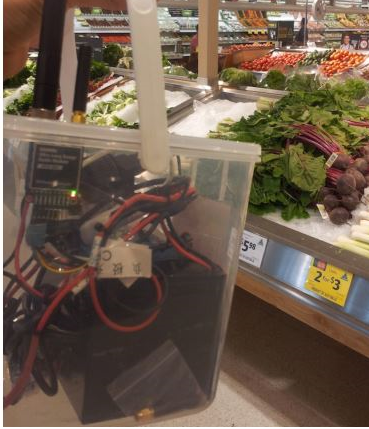
\includegraphics[width=0.3\textwidth]{image/meshextenderproto1.png}%
\caption{First prototype of the Mesh Extender (Gardner-Stephen et al., 2017a)}%
\label{figure:protoMesh}%-
\end{center}
\end{figure}


The Mesh Extender solved the two issues of the phone based solution and even bring a new advantage.
Since, they are creating, designing the Mesh Extender, they have a better control of the solution and less restriction. For instance, they were able to add other radio types such as a RFD900 (Gardner-Stephen et al., 2017a).



However, they quickly faced a major issue with this prototype. If you don't know it's a radio device, you may think it's a bomb. Hence, they add to work on the appearance of the Mesh Extender. Using 3-D printing, they created a new generation of the Mesh Extender:


\begin{figure}[H]
\begin{center}
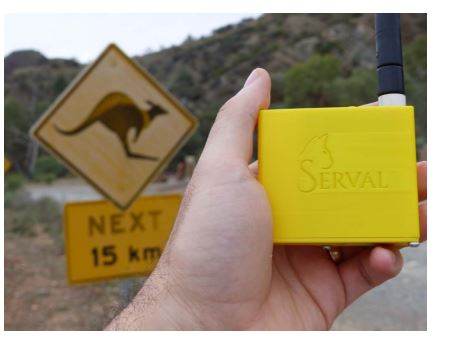
\includegraphics[width=0.4\textwidth]{image/meshextenderproto2.png}%
\caption{Seconde version of the Mesh Extender (Gardner-Stephen et al., 2017a)}%
\label{figure:protoMesh2}%-
\end{center}
\end{figure}


With this new generation, only the look changed. The component inside the Mesh Extender remained the same.
The last generation of the Mesh Extender changed that. It was design to have improved features and be ready for manufacture.


\begin{figure}[H]
\begin{center}
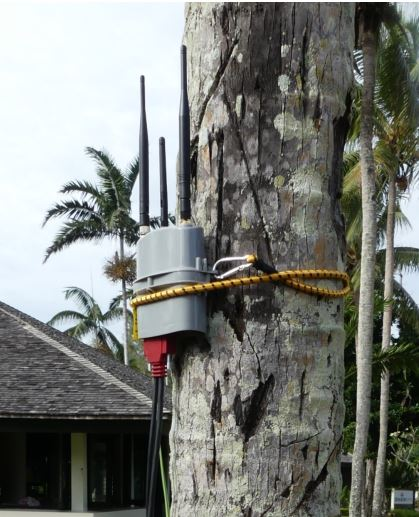
\includegraphics[width=0.4\textwidth]{image/meshextenderproto3.png}%
\caption{Latest version of the Mesh Extender in its natural environment (Gardner-Stephen et al., 2017a)}%
\label{figure:protoMesh3}%-
\end{center}
\end{figure}


The story of the Mesh Extender teaches us a lot for this project. First, the Mesh Extender is a product created years ago and that keeps evolving. When creating the test network, we have to think of the current features but also keep in mind that it may evolve or change in the future. 
The design of the Mesh Extender also gives us information on the philosophy behind the project. The team has a strong will to create affordable solutions using free open-software. The test network should reflect that philosophy.




\section{Pilot in Vanuatu}

Last year, the Serval team went to Vanuatu. A few conclusions were drawn from this trip. First, there is a strong need in Pacific nations for communication system such as the one proposed by the Serval project (Gardner-Stephen, 2017b). The Serval project is really interesting for Pacific nations like Vanuatu. First, since it is using solar power, it is self-sufficient. Second, the look of the product is rather professional. Finally, the Serval team is not a commercial for-profit operation(Gardner-Stephen, 2017b). 

Another goal of the trip in Vanuatu was to prove that the Serval Mesh Extender can work in a tropical-maritime environment (Gardner-Stephen, 2017b).

Finally, the last objective was to test the technology and find faults (Gardner-Stephen, 2018b).

Overall, the trip was a success. It proved that the Serval Mesh technology is working. But some faults were found and need to be fixed. All the data collected during the tests in Vanuatu will be very helpful to fix these faults. But in the long term, the team realised it will be beneficial to have a test network here at Tonsley. It could be used to understand the known faults and fix them but also to discover new ones.






\section{The current test network}
\subsection{Description of the test bed}


During the beginning of April, Paul installed an indoor test network at Tonsley.
The initial goal of this set-up was to verify if some bugs have been fixed. 

In the building, 13 points are linked to the Telecommunications Lab through copper and fibre. Therefore, we can easily place some Mesh Extenders at different location in the building. That's what Paul has done. 
At 4 different sites in the building, Paul installed one Mesh Extender. Hence, he created a multi-hop UHF network.

The repartition of the Mesh Extenders is the following:
\begin{itemize}
	\item 1 on the first floor
	\item 2 on the fourth floor
		\subitem 1 in the Telecommunications Lab
		\subitem 1 at the opposite side of the floor
	\item 1 on the fifth floor	
\end{itemize}
	

\begin{figure}[H]
	\centering
	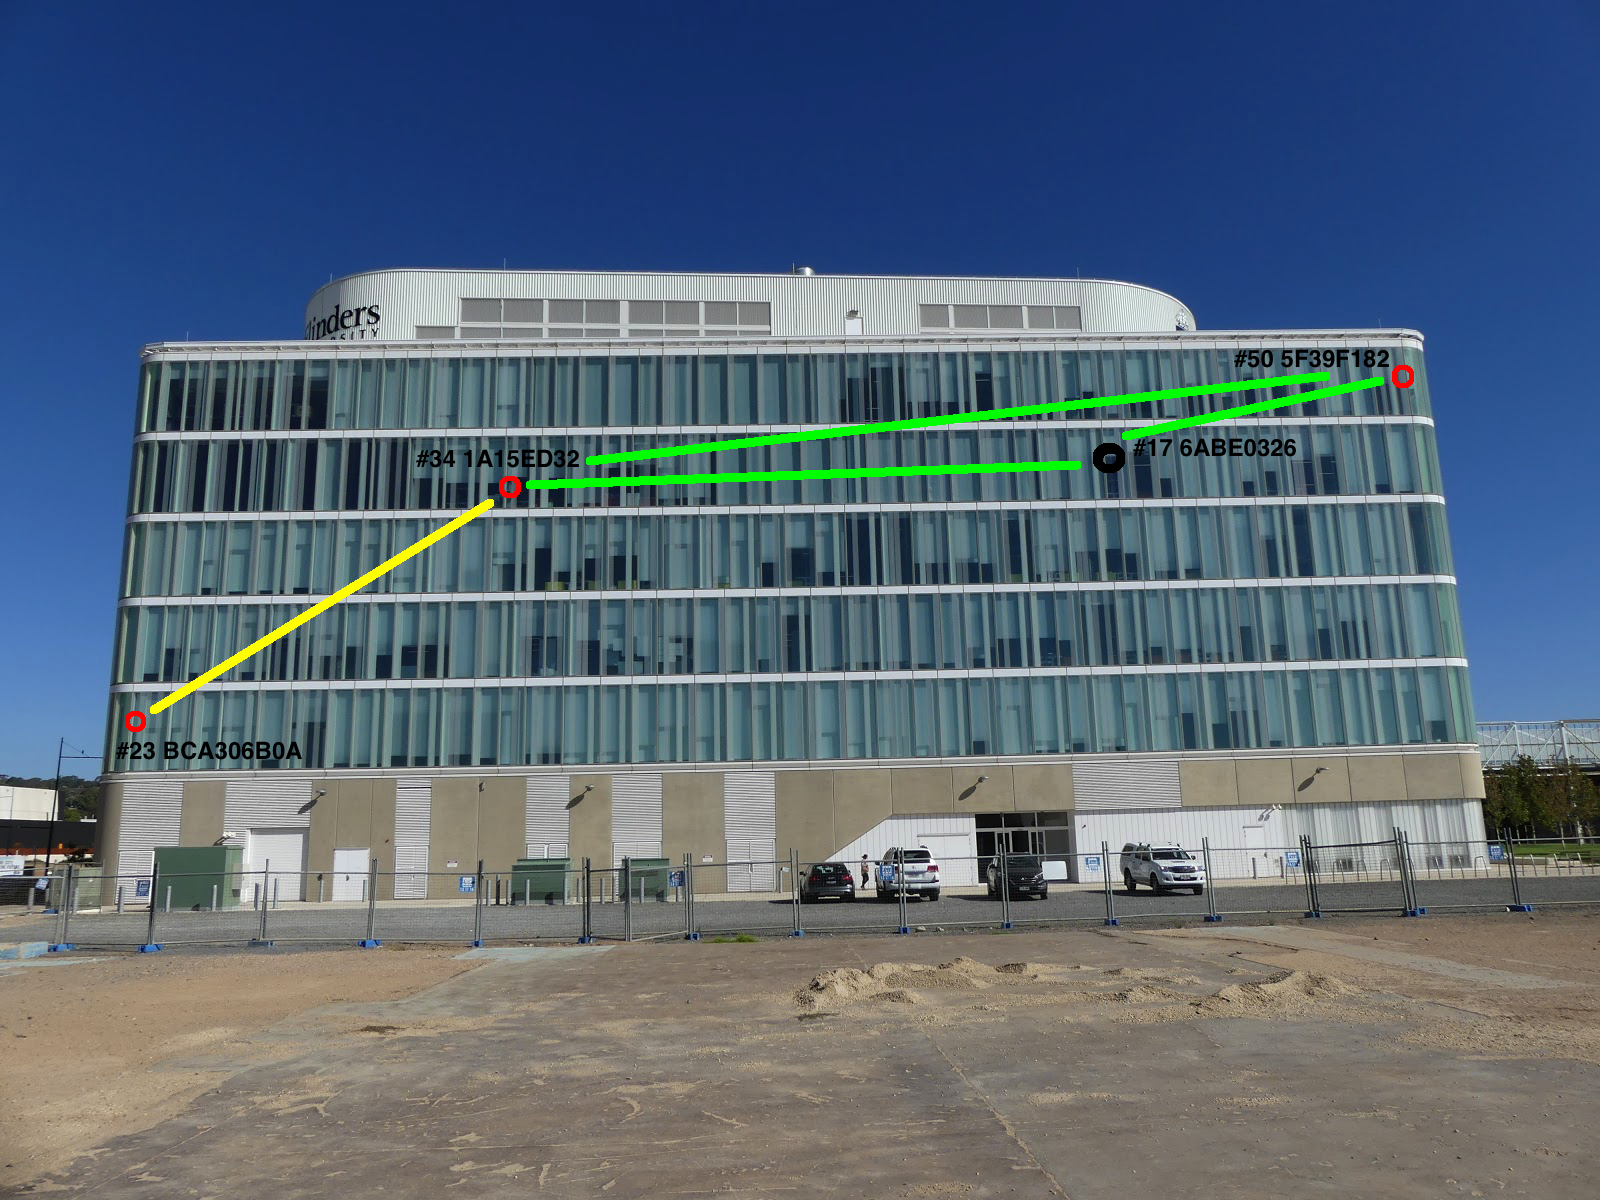
\includegraphics[width=0.6\textwidth]{image/TonsleyMeshExtenderLocations.png}
	\caption{Mesh Extender location (Gardner-Stephen, 2018a)}
	\label{fig:figure3}
\end{figure}


Since this network is supposed to be a multi-hop UHF, network, we want the Mesh Extenders to connect to each other using UHF and not Wi-Fi. For most of them, it is not a problem. Indeed, the Mesh Extenders are far enough from each other or the signal is heavily reduced by obstacles (walls for instance) for them to be able to connect with Wi-Fi.
However, the Mesh Extender on the fifth floor and one of the Mesh Extender on the fourth floor were able to communicate using Wi-Fi. Therefore, the Wi-Fi antenna was removed for one of the Mesh Extender(\#34 on the above picture).

With this set-up, we have a basic but functioning UHF network. We can use it to test some faults and fixes.


\subsection{Limitations of the current test network}

As explained previously, the current test network is made of 4 Mesh Extenders scattered across the building. This network is very basic and hence quick to install. However, it has some strong shortcomings.

The main issue with this network is its inconvenience. Indeed, this is just a UHF network, it doesn’t use Wi-Fi at all. Therefore, to test the network, you have to set-up a mobile at one of the site. Then move to another site and use a second phone to send a message to the first one. At the same time, you need to use computers to manually supervise each UHF link and each Wi-Fi connection involved in the communication. It can obviously be done but it will quickly become an hindrance to use repeatedly.

The second problem is the diversity. Since we only have Mesh Extenders on each site, we can only do basic test. If we want to do more complex tests, we need to go on each site to modify the set-up.

The last big problem is the current of short term improvement. Since the network is very basic, you cannot easily improve it. You cannot quickly add new features. You will need to add devices and heavily modify it to do so.



%%%%%%%%%%%%%%%%%%%%%%%%%%%%%%%%%%%%%%%%%%%%%%%%%%%
%								Next Section 											%
%%%%%%%%%%%%%%%%%%%%%%%%%%%%%%%%%%%%%%%%%%%%%%%%%%%
